%  LaTeX support: latex@mdpi.com
%  In case you need support, please attach any log files that you could have, and specify the details of your LaTeX setup (which operating system and LaTeX version / tools you are using).

%=================================================================

% LaTeX Class File and Rendering Mode (choose one)
% You will need to save the "mdpi.cls" and "mdpi.bst" files into the same folder as this template file.

%=================================================================

\documentclass[journal,article,accept,moreauthors,pdftex,12pt,a4paper]{mdpi}
%--------------------
% Class Options:
%--------------------
% journal
%----------
% Choose between the following MDPI journals:
% actuators, administrativesciences, aerospace, agriculture, agronomy, algorithms, animals, antibiotics, antibodies, antioxidants, appliedsciences, arts, atmosphere, atoms, axioms, batteries, behavioralsciences, beverages, bioengineering, biology, biomedicines, biomimetics, biomolecules, biosensors, brainsciences, buildings, cancers, catalysts, cells, challenges, chemosensors, children, chromatography, climate, coatings, computation, computers, cosmetics, crystals, data, dentistryjournal, diagnostics, diseases, diversity, econometrics, economies, education, electronics, energies, entropy, environments, epigenomes, fermentation, fibers, foods, forests, futureinternet, galaxies, games, gels, genealogy, genes, geosciences, geriatrics, healthcare, horticulturae, humanities, hydrology, informatics, information, inorganics, insects, ijerph, ijfs, ijms, ijns, ijgi, jcdd, jcm, jdb, jfb, jfmk, jimaging, jof, joi, jlpea, jmse, jpm, jrfm, jsan, land, languages, laws, life, lubricants, machines, marinedrugs, materials, mathematics, medicalsciences, membranes, metabolites, metals, microarrays, micromachines, microorganisms, minerals, molbank, molecules, nanomaterials, ncrna, nutrients, pathogens, pharmaceuticals, pharmaceutics, pharmacy, philosophies, photonics, plants, polymers, processes, proteomes, publications, recycling, religions, remotesensing, resources, risks, robotics, safety, sensors, sinusitis, socialsciences, societies, sports, standards, sustainability, symmetry, systems, technologies, toxics, toxins, universe, vaccines, veterinarysciences, viruses, water
%---------
% article
%---------
% The default type of manuscript is article, but could be replaced by using one of the class options:
% article, review, communication, commentary, bookreview, correction, addendum, editorial, changes, supfile, casereport, comment, conceptpaper, conferencereport, meetingreport, discussion, essay, letter, newbookreceived, opinion, projectreport, reply, retraction, shortnote, technicalnote, creative, datadescriptor (for journal Data), briefreport, hypothesis, interestingimage
%----------
% submit
%----------
% The class option "submit" will be changed to "accept" by the Editorial Office when the paper is accepted. This will only make changes to the frontpage (e.g. the logo of the journal will get visible), the headings, and the copyright information. Journal info and pagination for accepted papers will also be assigned by the Editorial Office.
% Please insert a blank line is before and after all equation and eqnarray environments to ensure proper line numbering when option submit is chosen
%------------------
% moreauthors
%------------------
% If there is only one author the class option oneauthor should be used. Otherwise use the class option moreauthors.
%---------
% pdftex
%---------
% The option "pdftex" is for use with pdfLaTeX only. If eps figure are used, use the optioin "dvipdfm", with LaTeX and dvi2pdf only.

%=================================================================
\setcounter{page}{1}
\lastpage{x}
\doinum{10.3390/------}
\pubvolume{xx}
\pubyear{2016}
%\externaleditor{Academic Editor: xx}
\history{Received: xx / Accepted: xx / Published: xx}

\usepackage{dsfont}
\usepackage[utf8]{inputenc}
\usepackage{algorithm}
\usepackage{amsmath}
\usepackage{amssymb}
\usepackage{algorithmicx}
\usepackage{algpseudocode}
\usepackage{natbib}

\DeclareUnicodeCharacter{00A0}{ }
\newcommand{\xx}{\boldsymbol{x}}
\newcommand{\dx}{d\boldsymbol{x}}
\newcommand{\data}{\boldsymbol{D}}
\newcommand{\II}{\boldsymbol{I}}

%------------------------------------------------------------------
% The following line should be uncommented if the LaTeX file is uploaded to arXiv.org
%\pdfoutput=1

%=================================================================

% Add packages and commands to include here
% The amsmath, amsthm, amssymb, hyperref, caption, float and color packages are loaded by the MDPI class.
%\usepackage{graphicx}
%\usepackage{subfigure,psfig}

%=================================================================
%% Please use the following mathematics environments:
% \theoremstyle{mdpi}
% \newcounter{thm}
% \setcounter{thm}{0}
% \newcounter{ex}
% \setcounter{ex}{0}
% \newcounter{re}
% \setcounter{re}{0}
%
% \newtheorem{Theorem}[thm]{Theorem}
% \newtheorem{Lemma}[thm]{Lemma}
% \newtheorem{Corollary}[thm]{Corollary}
% \newtheorem{Proposition}[thm]{Proposition}
%
% \theoremstyle{mdpidefinition}
% \newtheorem{Characterization}[thm]{Characterization}
% \newtheorem{Property}[thm]{Property}
% \newtheorem{Problem}[thm]{Problem}
% \newtheorem{Example}[ex]{Example}
% \newtheorem{ExamplesandDefinitions}[ex]{Examples and Definitions}
% \newtheorem{Remark}[re]{Remark}
% \newtheorem{Definition}[thm]{Definition}
%% For proofs, please use the proof environment (the amsthm package is loaded by the MDPI class).

%=================================================================

% Full title of the paper (Capitalized)
\Title{Nested sampling with two objective functions}

% Authors (Add full first names)
\Author{Brendon J. Brewer$^{1,}$*, Ewan Cameron$^{2}$, and
Robert J. N. Baldock$^{3}$}

% Affiliations / Addresses (Add [1] after \address if there is only one affiliation.)
\address{%
$^{1}$ Department of Statistics, The University of Auckland, Private Bag 92019,
Auckland 1142, New Zealand\\
$^{2}$ Spatial Ecology and Epidemiology Group, Tinbergen Building, Department
of Zoology, University of Oxford, South Parks Road, Oxford, UK\\
$^{3}$ Cavendish, University of Cambridge, Cambridge, UK}

%\contributed{$^\dagger$ These authors contributed equally to this work.}

% Contact information of the corresponding author (Add [2] after \corres if there are more than one corresponding author.)
\corres{{\tt bj.brewer@auckland.ac.nz}}

% Abstract (Do not use inserted blank lines, i.e. \\)
\abstract{We present a generalization of the Nested Sampling algorithm for
estimating the partition function $Z(\beta_1, \beta_2)$ of a family of
probability distributions indexed by two hyperparameters $\beta_1$ and
$\beta_2$. These
problems arise frequently in statistical mechanics and occasionally in
Bayesian inference. We demonstrate the algorithm on a toy example where
$Z(\beta_1, \beta_2)$ is known, and show empirically that the accuracy
improves as XX as a function of the number of particles $N$. We also
calculate the partition function for a Lennard-Jones system in an external
field, as a function of the external field strength, in a single run.}

% Keywords: add 3 to 10 keywords
\keyword{nested sampling; bayesian computation; statistical mechanics}

% The fields PACS, MSC, and JEL may be left empty or commented out if not applicable
%\PACS{}
%\MSC{}
%\JEL{}

% If this is an expanded version of a conference paper, please cite it here: enter the full citation of your conference paper, and add $^\dagger$ in the end of the title of this article.
%\conference{}

%%%%%%%%%%%%%%%%%%%%%%%%%%%%%%%%%%%%%%%%%%
% For journal Data:

%\dataset{DOI number or link to the deposited data set in cases where the data set is published or set to be published separately. If the data set is submitted and will be published as a supplement to this paper in the journal Data, this field will be filled by the editors of the journal. In this case, please make sure to submit the data set as a supplement when entering your manuscript into our manuscript editorial system.}
%\datasetlicense{license under which the data set is made available (CC0, CC-BY, CC-BY-SA, CC-BY-NC, etc.)}

%%%%%%%%%%%%%%%%%%%%%%%%%%%%%%%%%%%%%%%%%%

\begin{document}

%%%%%%%%%%%%%%%%%%%%%%%%%%%%%%%%%%%%%%%%%%

\section{Introduction}

Nested Sampling \citep[NS][]{skilling} is popular general
Monte Carlo algorithm that can solve a wide range of problems in Bayesian
computation and statistical mechanics
\citep{2009arXiv0906.3544P, 2014PhRvE..89b2302P, 2015arXiv150303404B}.
Its key strength its ability to cope with phase transitions which cause
many other methods to fail.
In a Bayesian inference framework with unknown parameters denoted collectively
by a vector $\xx$, the
posterior distribution for the parameters given data $\data$ (and prior
information $\II$) is:
\begin{eqnarray}
p(\xx | \data, \II) &=&
\frac{p(\xx | \II)p(\data | \xx, \II)}{p(\data | \II)}\\
&=& \frac{\pi(\xx)L(\xx)}{Z}
\end{eqnarray}
where $\pi(\xx)$ is the prior distribution, $L(\xx)$ is the likelihood
function, and $Z$ is the normalising constant, usually known as the
`marginal likelihood' or the `evidence':
\begin{eqnarray}
Z &=& \int \pi(\xx) L(\xx) \, \dx.\label{eqn:evidence}
\end{eqnarray}

$Z$ is useful because it is the probability of the data given that
$\xx$ is {\em one of}
the possibilities in the space being integrated over, and thus plays the role
of a likelihood for the parameter space as a whole.
The main goal of NS is to approximate $Z$, but it can also be used to make
Monte Carlo approximations of the posterior distribution, and to
calculate the `information',
or Kullback-Leibler divergence from the prior to the posterior:
\begin{eqnarray}
\mathcal{H} &=& \int p(\xx | \data, \II) \ln
\left[\frac{p(\xx | \data, \II)}{p(\xx | \II)}\right] \, d\xx \\
&=& \int \frac{\pi(\xx) L(\xx)}{Z} \ln
\left[\frac{L(\xx)}{Z}\right] \, d\xx.
\end{eqnarray}
$\mathcal{H}$ quantifies how compressed the posterior distribution is with
respect to the prior. For example, $\mathcal{H} = 10$ implies (loosely speaking)
that the posterior occupies a fraction $e^{-10}$ of the prior mass.
$\mathcal{H}$ can be interpreted quite literally as a measure of how much
the data $\data$ told you about $\xx$.

NS works by drawing particles from the
prior $\pi(\xx)$ and successively imposing constraints on the value of
the likelihood $L(\xx)$ that compress the prior mass by a (roughly) known
and constant factor. Like related algorithms such as those
based on `annealing' or `tempering', NS
moves through a sequence of probability distributions beginning from the
prior. This sequence of distributions is defined by
\begin{eqnarray}
p(\xx; \ell) &=& \frac{1}{X(\ell)}\pi(\xx)\mathds{1}\left(L(\xx) > \ell\right).
\label{eq:constrained_prior}
\end{eqnarray}
and the marginal likelihood can be computed by numerically integrating the
function $L(X)$:
\begin{eqnarray}
Z &=& \int_0^1 L(X)\, dX.
\end{eqnarray}
Throughout this paper we use the popular `overloaded' notation for some
functions and probability distributions.
For example, $L(\xx)$ is the likelihood function, and $L(X)$ is the likelihood
as a function of the enclosed prior mass $X$. These cannot literally be the
same function as the inputs are not even necessarily of the same dimensionality.
Therefore the symbol $L$ implies that the output of the function is a
likelihood value; so $L(\xx)$ represents a likelihood value computed from
the parameters $\xx$, and $L(X)$ represents a likelihood value that
corresponds to an amount $X$ of prior mass.

Naively, Equation~\ref{eqn:evidence} appears straightforward to compute because
it is a simple expectation of $L$ with respect to the distribution $\pi$.
However,
NS is required because Equation~\ref{eqn:evidence}
is the expected value of $L$ with respect to a very heavy-tailed distribution
(the prior for the $L$ value implied by $\pi(\xx)$). Hence, there is a strong
connection between NS and ideas from rare event simulation, which has been
explicitly investigated by \citet{walter}.

Using a single NS run, we can also calculate the properties of any other distribution that
is in some sense intermediate
between the prior and the posterior. For example, we might be interested in
a `power posterior' where the likelihood is raised to a power $\beta$:
\begin{eqnarray}
p(\xx; \beta) &=& \frac{\pi(\xx)L(\xx)^\beta}{Z(\beta)}\label{eqn:power_posterior}
\end{eqnarray}
The normalisation and posterior samples from this distribution can be obtained
from the original NS run by re-weighting the output according to $L(\xx)^\beta$
instead of the usual $L(\xx)$ used to obtain the posterior.
An example application, in the case of
a Bayesian inference problem with a `gaussian noise' likelihood assumption,
computing $p(\xx; \beta)$ for $\beta \neq 1$ allows us to explore what the
posterior distribution would have been if the noise variance had been greater,
without having to re-run the algorithm.
This is different from including an extra parameter to allow the noise variance
to be greater, because NS allows you to test the consequences of values of the
variance that are very implausible given the data.

Alternatives to NS include methods based on `annealing', where a sequence of
distributions of the form of Equation~\ref{eqn:power_posterior} is used.
There are many different methods based on this idea, such as the popular
parallel tempering method \citep{pt, gregory}.
However, unlike annealing methods, NS requires only a small number of
tuning parameters (just the number of particles $N$ is inherent to NS, although
most NS implementations also have some tuning parameters related to their
methods for sampling Equation~\ref{eq:constrained_prior}). Annealing methods
also tend to fail on phase change problems \citep{skilling} which can arise
in data analysis \citep{rjobject, exoplanet}.

In statistical mechanics, Equation~\ref{eqn:power_posterior} defines the
family of {\it canonical distributions}, usually written as:
\begin{eqnarray}
p(\xx; \beta) &=& \frac{\pi(\xx)\exp[-\beta E(\xx)]}{Z(\beta)}
\end{eqnarray}
where $E(\xx)$ is the energy function (analogous to minus the log likelihood
in the Bayesian case), and $\pi(\xx)$ is often uniform over
phase space (the set of possible positions and momenta of a collection of
particles) or configuration space (the set of possible positions of a collection
of particles). In this context we usually want to
compute $Z(\beta)$ as a function of $\beta$, which is called the
{\it partition function}. The quantity $\mathcal{I}(\beta)$ is, up to a sign
change and an additive constant, the Gibbs entropy.
NS can achieve this, allowing the study of
the properties of materials from first principles, based on hypotheses about
the atoms or molecules that make them up \citep[e.g.][]{2009arXiv0906.3544P,
2014PhRvE..89b2302P, 2015arXiv150303404B}. The NS algorithm is invariant under
monotonic transformations of $L$ or $E$ and therefore there we can discuss the
algorithm in Bayesian or statistical mechanical terms without loss of
generality.

Throughout this paper we will refer to $L(\xx)$ or
$-E(\xx)$ as `objective functions',
by analogy with the terminology used when
discussing optimization methods. Although we are interested in sampling rather
than optimization, we still want to increase the values of $L$ or decrease
the values of $E$ relative to what is typical of the prior.

In some inference and
statistical mechanics problems, there are two or more scalar functions of
$\xx$ that are relevant. Suppose our prior is $\pi(\xx)$ as before, and
we obtain information that fixes the expected values of two scalar
functions of $\xx$, $L_1(\xx)$ and $L_2(\xx)$.
It is well known that the
updated probability distribution that takes into account the constraints is
of the canonical form:
\begin{eqnarray}
p(\xx; \beta_1, \beta_2) &=& \frac{\pi(\xx)\exp\left[\beta_1L_1(\xx)+\beta_2L_2(\xx)\right]}
{Z(\beta_1, \beta_2)}
\end{eqnarray}
where $\beta_1$ and $\beta_2$ are two `inverse temperatures' (the temperatures
themselves are $T_1 = \beta_1^{-1}$ and $T_2 = \beta_2^{-1}$).
In a Bayesian
context, this distribution (when $\beta_1 = \beta_2 = 1$) could be the
posterior distribution for parameters $\xx$
given two datasets, where $L_1$ and $L_2$ are the
likelihood functions for each dataset. In statistical mechanics, $L_1$ might
be $\exp\left(-\textnormal{energy}\right)$ and $L_2$ might be the total
angular momentum, or be a term depending on an external field (so $\beta_2$
would then describe the strength of the external field).

If we are only interested in a single canonical distribution, for example
with $\beta_1 = 0.3$ and $\beta_2 = 0.7$, we can estimate its normalising
constant and by running standard Nested Sampling with objective function
$L(\xx) = \exp\left[0.3L_1(\xx) + 0.7L_2(\xx)\right]$. However, usually we
are interested in a range of values for $\beta_1$ and $\beta_2$, and we
want to know the entire partition function $Z(\beta_1, \beta_2)$.
This work describes
progress towards solving this class of problems while maintaining the benefits
of Nested Sampling, such as the ability to cope with first-order phase
transitions. The algorithm is designed for problems with two objective
functions, but may generalize to problems with more than two (though perhaps
not more than a few).

The prior $\pi(\xx)$ implies a certain prior for $L_1$ and $L_2$, which we
denote $\pi(L_1, L_2)$. An example of a prior is shown as the
probability density in Figure~\ref{fig:joint1}. The partition function
$Z(\beta_1, \beta_2)$ is a set of expected values with respect to this density.
Simple Monte Carlo sampling from $\pi$ will not work except for values of
$(\beta_1, \beta_2)$ where the canonical distribution remains similar to $\pi$.
We need a sampler that explores regions where $L_1$ and $L_2$ are high in order
to accurately estimate $Z(\beta_1, \beta_2)$.
\begin{figure}
\centering
\includegraphics[scale=0.5]{figures/joint1.pdf}
\caption{\it An example of a prior for $L_1$ and $L_2$, which is implied by
the prior $\pi(\xx)$. We have overplotted 25 points drawn from this prior.
The estimated prior mass in the shaded rectangle is
$\hat{X}(2, 1.5) = 5/25 = 0.2$.
\label{fig:joint1}}
\end{figure}

Our proposed algorithm (introduced in Section~\ref{sec:algorithm}) makes use
of the (two dimensional) cumulative distribution of the objective functions.
For any values $(\ell_1, \ell_2)$ of the objective functions,
the prior mass for which both $L_1 \geq \ell_1$ {\em and} $L_2 \geq \ell_2$ is:
\begin{eqnarray}
X(\ell_1, \ell_2) &=& \int \pi(L_1, L_2)
\mathds{1}\left[L_1 \geq \ell_1, L_2 \geq \ell_2 \right]
 \, dL_1 \, dL_2.
\end{eqnarray}
Since $X$ is a probability, it must satisfy a product rule:
\begin{eqnarray}
X(\ell_1, \ell_2) = X(\ell_1)X(\ell_2 | \ell_1) = X(\ell_2)X(\ell_1 | \ell_2).
\end{eqnarray}

When the prior $\pi$ is approximated with a set of $N$
particles $\{\xx_i\}_{i=1}^N$
(Monte Carlo samples ``drawn from'' $\pi$),
$X(\ell_1, \ell_2)$ can be approximated by:
\begin{eqnarray}
\hat{X}(\ell_1, \ell_2) &=&
\frac{1}{N}
\sum_{i=1}^N \mathds{1}\left[L_1(\xx_i) \geq \ell_1,
L_2(\xx_i) \geq \ell_2\right].\label{eqn:corner_count}
\end{eqnarray}
Graphically, on a plot of $L_2$ vs. $L_1$, $\hat{X}(\ell_1, \ell_2)$
is the fraction of particles in the rectangle whose upper right corner is at
$\left(\ell_1, \ell_2\right)$. See Figure~\ref{fig:joint1} for an
example.

\section{Properties of Nested sampling}

We seek an algorithm for computing the partition function
$Z(\beta_1, \beta_2)$ for a range of values of the $\beta$s, from a single
run. To be a variant of Nested Sampling, the algorithm should satisfy
the following properties:
\begin{enumerate}
\item It should begin with $N$ points drawn from the prior $\pi(\xx)$.
\item It should seek to explore regions where the values of
$L_1(\xx)$ and $L_2(\xx)$ are higher than the prior $\pi(L_1, L_2)$
would typically imply.
\item The algorithm should consider a sequence of probability
distributions proportional to $\pi$, but restricted to smaller and smaller
domains for which the enclosed prior mass shrinks by a (roughly) constant and
known factor each iteration.
\item The algorithm should be invariant to monotonic transformations of
$L_1$ and $L_2$, i.e. it should only depend on rankings of $L_1$ and $L_2$
values and not the values themselves.
\end{enumerate}
The standard Nested Sampling algorithm has these properties but for a
single objective function. The same is true of variants such as
Diffusive Nested Sampling \citep{dnest}.

\section{Rationale}\label{sec:rationale}

Consider the following proposal, which we label the `turn-the-corner idea'.
Imagine running standard NS with $N$ particles
using the objective function $L_1(\xx)$.
After $M_1$ iterations, we'd be able to approximate
the function $X(\ell_1) = \int \pi(\xx) \, d\xx$
from $X\approx e^{-M_1/N}$ to $X=1$. Defining $Y=-\ln(X)$, we could also
construct an approximation to the function
$L_1(Y)$, a non-decreasing function of $Y$, from $Y=0$ to $Y\approx M_1/N$.
After $M$ iterations, we keep the last value of $L_1(\xx)$ obtained
(call it $L_1^*$), and continue to impose the constraint $L_1(\xx) > L_1^*$.

Subject to the constraint $L_1(\xx) > L_1^*$, standard NS can continue but
attempting to increase $L_2$ instead of $L_1$. This is what we mean by
`turning the corner'. After $M_2$ such iterations,
the algorithm would have compressed the prior by a factor
$e^{(M_1 + M_2)/N}$ and therefore ended at a point in the $(L_1, L_2)$ plane
where $X(L_1, L_2) \approx e^{-(M_1 + M_2)/N}$. Any such run consisting of
$M_1 + M_2$ iterations will therefore appoximately finish on a contour line
of the function $X(L_1, L_2)$.
We have explored the idea of using multiple turn-the-corner runs, with
the corner being turned at different times (i.e. using different values of
$M_1$), and combining the results using biased sampling
\citep{vardi, cameron} in order to estimate $Z(\beta_1, \beta_2)$. However,
this was very computationally intensive. We presented the turn-the-corner idea
here in order to provide an intuitive rationale for our actual algorithm given in
Section~\ref{sec:algorithm}.

Figure~\ref{fig:contours} shows the contour lines of $X(L_1, L_2)$ for the
prior in Figure~\ref{fig:joint1}. Each contour line encloses half of the
prior mass of the previous one. The fact that contours of $X(L_1, L_2)$ are
relevant suggests that a standard NS run with objective function
$X(L_1(\xx), L_2(\xx))$ would achieve a similar effect to the turn-the-corner
idea.

\begin{figure}
\centering
\includegraphics[scale=0.5]{figures/contours.pdf}
\caption{\it The joint prior for the objective functions, and fifteen
contours of the cumulative distribution $X(L_1, L_2)$, each enclosing half
the prior mass of the previous one. \label{fig:contours}}
\end{figure}

{\bf Try to relate this to \citet{vertical}}.

\section{Proposed algorithm}\label{sec:algorithm}

The basic idea of our algorithm is to try to mimic a standard NS run, where the
objective function being increased is
\begin{eqnarray}
Y(\xx) &=& 1/X\left(L_1(\xx), L_2(\xx)\right).
\end{eqnarray}
Standard NS cannot be applied simply because we cannot evaluate $X(L_1, L_2)$ and
therefore cannot restrict the parameter space based on the value of $X$ (or
equivalently, $Y$). However, given a number of Monte Carlo samples, we
can {\em approximate} $X$ by $\hat{X}(L_1, L_2)$, and restrict the parameter
space based on a contour of that approximation.
The algorithm is presented in detail below.

\begin{algorithm}[ht!]
\begin{algorithmic}
\State 1) Generate $N$ particles $\{\xx_1, ..., \xx_N\}$ from $\pi(\xx)$.
$N$ should quite large (typically 1000 or greater), and the algorithm is
slightly more elegant if $N$ is odd.
\State 2) Initialise the {\em remaining prior mass} to be $M=1$.
\State 3) Initialise the {\em excluded region} $\mathcal{R}$ to be the empty set
$\emptyset$.
\While{more iterations desired}
	\State i) Calculate $\hat{X}(\ell_1, \ell_2)$ at the position of each particle
			and sort the $\hat{X}$ values observed.
	\State ii) Find the median $\hat{X}$ value, $\hat{X}_{(k)}$.
	\State iii) Classify all particles as either ``interior'', ``boundary'', or
			``exterior'', based on whether their $\hat{X}$ values are
			greater than, equal to, or less than $\hat{X}_{(k)}$ respectively.
	\State iv) If the number of interior particles $n_{\rm interior}$ or the number
			of exterior particles $n_{\rm exterior}$ is zero, replace $k$ by
			$(k-1)$ (to try a percentile other than the median)
			and go to step iii) (if $k=1$ then set $k=N$ instead of zero).
	\State v) Save all ``interior'' particles to disk, assigning each a prior weight of $n_{\rm interior}/(n_{\rm interior} + n_{\rm exterior})$.
	\State vi) Exclude the region in the $L_1$-$L_2$ plane where
$\hat{X} \geq \hat{X}_{(k)}$. That is, set
	\State \hspace{20pt} $\mathcal{R} \leftarrow \mathcal{R} \cup \{(\ell_1, \ell_2) \in \mathbb{R}^2: \hat{X}(\ell_1, \ell_2) \geq \hat{X}_{(k)}\}$.
	\State vii) Update the remaining prior mass to $M \leftarrow M n_{\rm exterior}/N$.
	\State viii) Replace all interior and boundary particles by new
			particles generated from $\pi(\xx)$, subject to the constraint
			of not being in the excluded region.
\EndWhile
\end{algorithmic}
\caption{\label{alg:algorithm}}
\end{algorithm}

%Step 1 of the algorithm ensures that NS property 1 is trivially satisfied.

\begin{figure}
\centering
\includegraphics[scale=0.5]{figures/joint2.pdf}
\caption{\it The joint prior for the objective functions, and Monte Carlo
samples, as in Figure~\ref{fig:joint1}. The shaded region imposes a
constraint on the value of $\hat{X}$. Its boundary approximates a contour
of $X(L_1, L_2)$.
\label{fig:joint2}}
\end{figure}

\section{Example 1: Known solution}
We tested the algorithm on a simple 100-dimensional example, where the
prior is a uniform distribution between 0 and 1 for each coordinate:
\begin{eqnarray}
\pi(\xx) &=& \prod_{i=1}^{100}
\left\{
\begin{array}{lr}
1, & x_i \in [0, 1]\\
0, & \textnormal{otherwise.}
\end{array}
\right.
\end{eqnarray}
The first objective function is quadratic in form, such that the canonical
distribution is an iid gaussian centered at $(0.5, 0.5, ..., 0.5)$:
\begin{eqnarray}
L_1(\xx) &=& -\sum_{i=1}^{100} \left(x_i - 0.5\right)^2.
\end{eqnarray}

The second objective function upweights states where coordinates $\{x_i\}$
are close to 0, 0.25, 0.5, 0.75, or 1:
\begin{eqnarray} 
L_2(\xx) &=& -\sum_{i=1}^{100} \sin^2(4\pi x_i)
\end{eqnarray}

The true partition function (computed numerically) and the Kullback-Leibler
divergence from the prior to the canonical distribution are shown in
Figure~\ref{fig:truth} as a function of two temperatures.

\begin{figure}
\centering
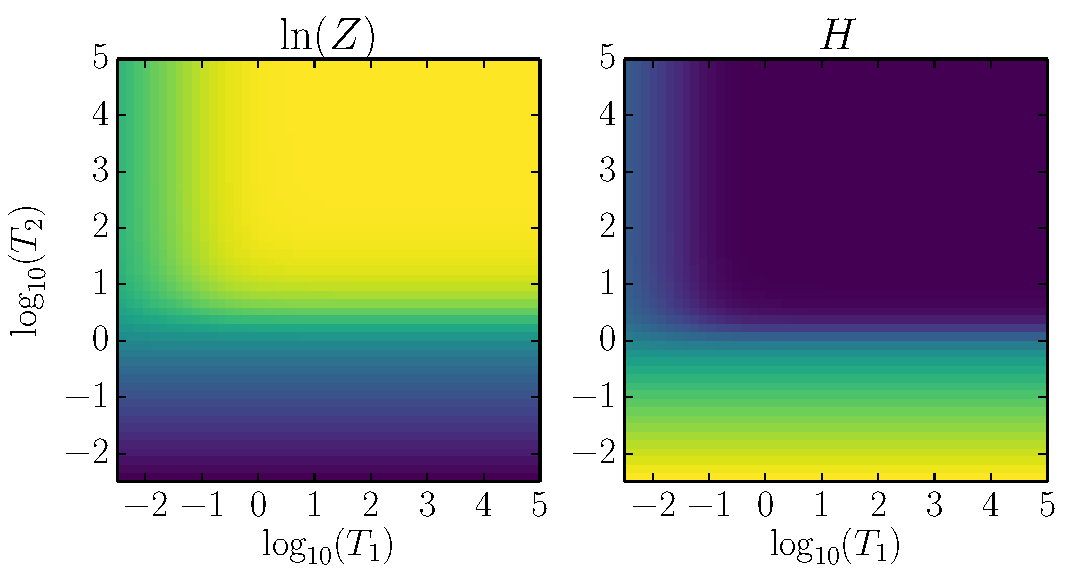
\includegraphics[scale=0.75]{figures/truth.pdf}
\caption{The true partition function and KL divergence (from the prior to
the canonical distribution) as a function of two temperatures for the
test problem.\label{fig:truth}}
\end{figure}


\begin{figure}
\centering
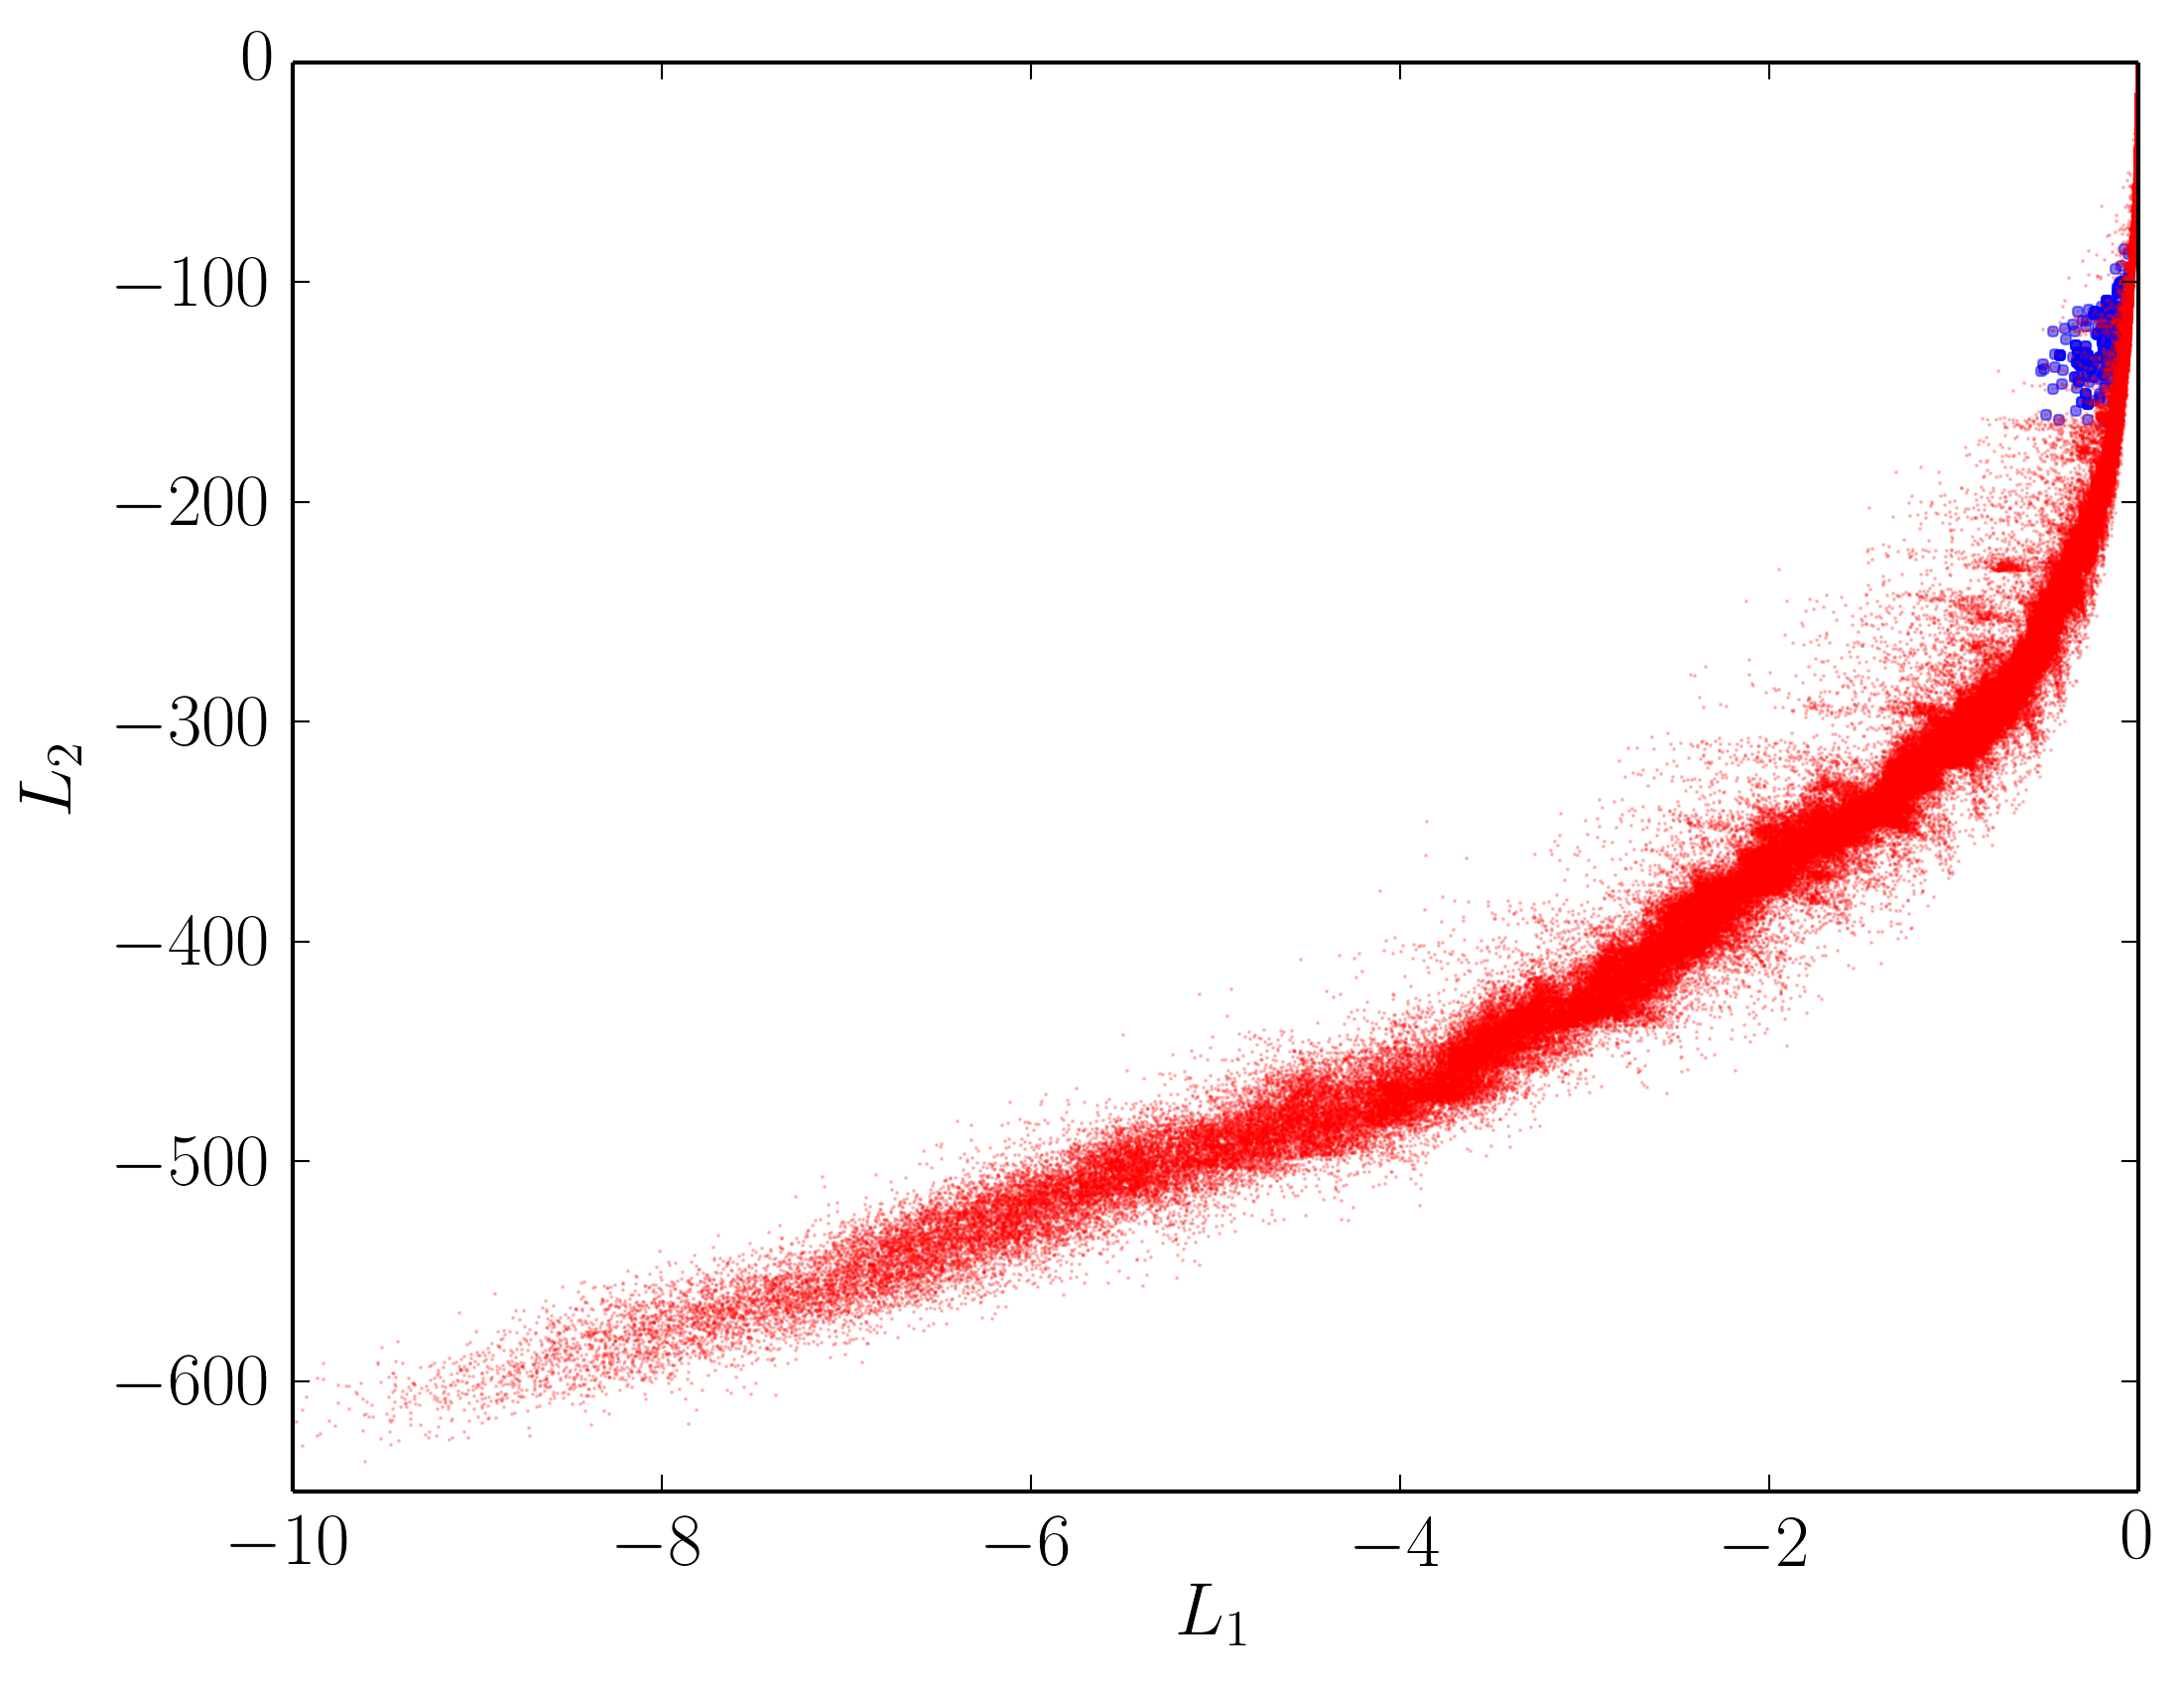
\includegraphics[scale=0.75]{figures/output.png}
\caption{The sequence of discarded particles (yellow) and
points representing the canonical distribution at temperatures
$(T_1, T_2) = (0.1, 1)$ (black).\label{fig:output}}
\end{figure}



\begin{figure}
\centering
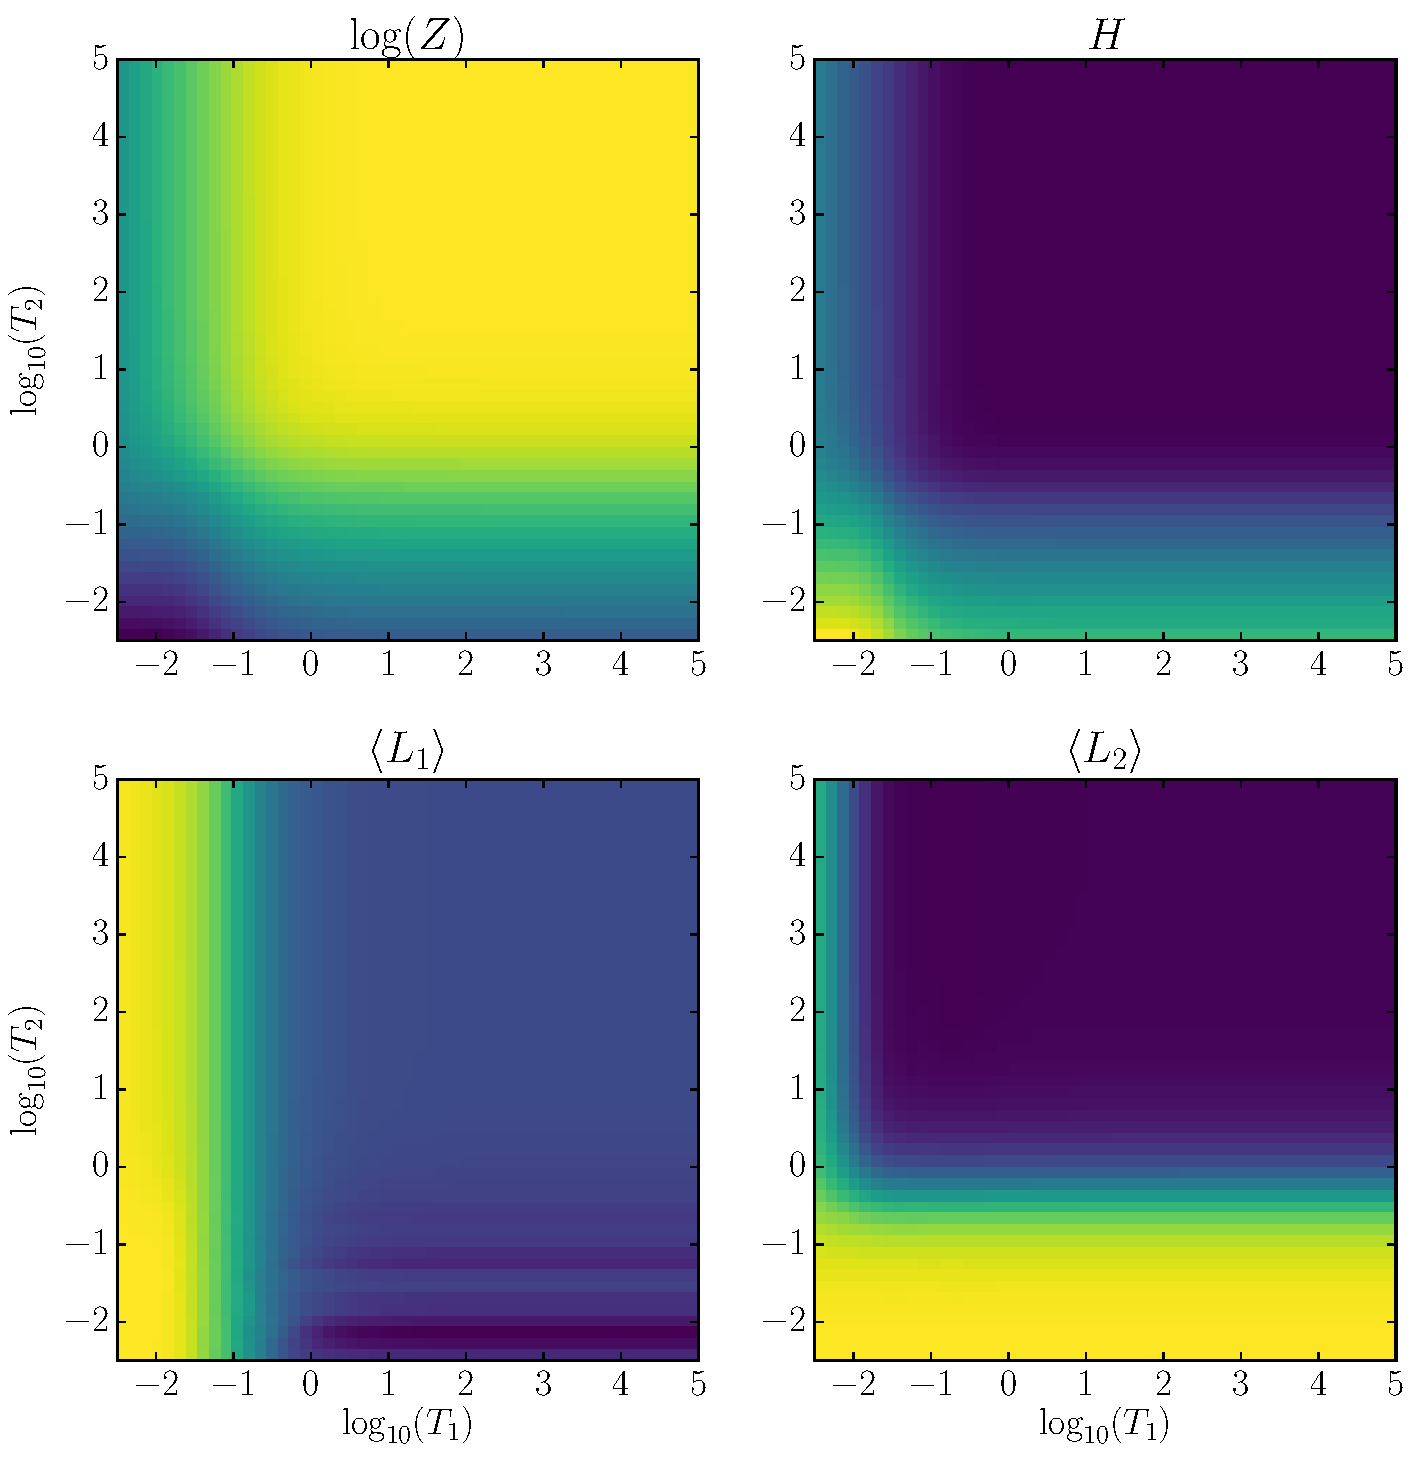
\includegraphics[scale=0.5]{figures/results.pdf}
\caption{Numerical results for the test problem. These compare well with the
true partition function and KL divergence given in Figure~\ref{fig:truth}.
\label{fig:results}}
\end{figure}

\section{Example 2: Lennard-Jones/Polymer Example}



\section{Example 3: ``MaxEnt'' image deconvolution example}
Problems with more than one objective function can also arise in data
analysis. Consider, for example, the problem of deblurring a noisy
image. A common approach to these problems is regularized inversion,
such as the ``maximum entropy'' technique of \citet{gull}. It is important
to distinguish between this method and the maximum entropy principle used
to update or assign probabilities \citep{caticha}.

The unknown parameters are a set of pixel intensities
$\{m_i\}_{i=1}^n$ where $n$ is the number of pixels and $m_i \geq 0$.
The dataset is also a collection of pixel intensities $\{D_i\}_{i=1}^n$.
The prior for the dataset given the parameters is a normal distribution
with mean given by the underlying image $\{m_i\}$ convolved by
a point spread function. The standard deviation of each pixel is
$\sigma$, assumed known. This is usually written as

\begin{eqnarray}
\boldsymbol{D} = \boldsymbol{P}\boldsymbol{m} + \boldsymbol{n}
\end{eqnarray}
where $\boldsymbol{n}$ is the noise in each pixel and $\boldsymbol{P}$ is
the blurring operator written in matrix form.

The posterior for the underlying image given the data is
\begin{eqnarray}
p(\boldsymbol{m} | \boldsymbol{D})
&=& \frac{p(\boldsymbol{m})p(\boldsymbol{D}|\boldsymbol{m})}
{\int p(\boldsymbol{m})p(\boldsymbol{D}|\boldsymbol{m}) \,d^n\boldsymbol{m}}\\
&=& \frac{\exp\left[-\lambda \sum_i m_i\ln m_i
-\frac{1}{2\sigma^2}\left(D_i - \sum_{j} P_{ij}m_{j}\right)^2\right]}
{\int \exp\left[-\lambda \sum_i m_i\ln m_i
-\frac{1}{2\sigma^2}\left(D_i - \sum_{j} P_{ij}m_{j}\right)^2\right]\, d^n\boldsymbol{m}}
\end{eqnarray}


Therefore, this is a `doubly intractable' problem, closely related to
those studied (and solved) by \citep{murray}.

\section{What kind of accuracy can we expect?}

Imagine computing $Z(\beta_1, \beta_2)$ by looping over a grid of $\beta_2$
values and doing an NS run with respect to $L_1$ for each. For each
value of $\beta_1$ and $\beta_2$ that we're interested in, we can expect
a (marginal) `one-sigma' accuracy in
$\ln\left[Z(\beta_1, \beta_2)\right]$ of $\pm \sqrt{H(\beta_1, \beta_2)/N}$,
for a computational cost proportional to...

\section{What kind of accuracy do we need?}

The following argument is due to John Skilling. Consider Bayesian model selection
between two models $M_1$ and $M_2$. The Bayes Factor is the ratio of the
two marginal likelihoods:
\begin{eqnarray}
B = \frac{P(D | M_1)}{P(D | M_2)} = \frac{Z_1}{Z_2}
\end{eqnarray}
where $Z_1 = \int \pi(\xx_1)L(\xx_1) \, d\xx_1$ and
$Z_2 = \int \pi(\xx_2)L(\xx_2) \, d\xx_2$.
In large problems, the log of the Bayes Factor is usually more convenient:
\begin{eqnarray}
\Delta := \ln B = \ln Z_1 - \ln Z_2.
\end{eqnarray}
Naively, we want $\Delta$ to an accuracy of about 0.1, so that we can reliably
quantify the strength of the evidence when the two models are similarly
supported by the data. But is this a realistic situation?

Prior to knowing the data $D$, we don't know how much information we will get
about the question of $M_1$ vs. $M_2$, quantified by the KL divergence:
\begin{eqnarray}
\mathcal{H} &=& \sum_{i=1}^2 P(M_i | D)
\ln\left[
\frac{P(M_i | D)}{P(M_i)}
\right].
\end{eqnarray}

The expected value of $\mathcal{H}$ (with respect to the prior over datasets)
is the mutual information:
\begin{eqnarray}
\mathcal{I} &=& \mathds{E}\left[\mathcal{H}\right]\\
&=&
\sum_{i=1}^2 \int P(M_i, D)
\ln\left[
\frac{P(M_i, D)}{P(M_i)P(D)}
\right] \, dD.
\end{eqnarray}

\section{Failure modes}\label{sec:failure_modes}

If $L_1(\xx)$ and $L_2(\xx)$ are inversely and strongly dependent...


%Use Skilling's argument about the prior distribution of a log Bayes factor.
%Even though the performance of this algorithm won't be great for high $H$, it
%will be good enough. I think the probability it won't give enough accuracy will
%be ``exponentially small''.

\acknowledgments{Acknowledgements}

It is a pleasure to thank Gábor Csányi (Cambridge), Livia B. Pártay (Cambridge),
and Will Handley (Cambridge)
for valuable conversations.

%%%%%%%%%%%%%%%%%%%%%%%%%%%%%%%%%%%%%%%%%%

\authorcontributions{Author Contributions}

BJB initiated the project and explored various ideas which did not work.
EC worked on the biased sampling suggestion in Section~\ref{sec:rationale},
discovered the failure mode in Section~\ref{sec:failure_modes}, ...
%%%%%%%%%%%%%%%%%%%%%%%%%%%%%%%%%%%%%%%%%%

\conflictofinterests{Conflicts of Interest}
The authors declare no conflict of interest.

%=================================================================
% References: Variant A
%=================================================================
% Back Matter (References and Notes)
%----------------------------------------------------------
% Style and layout of the references
\bibliographystyle{mdpi}
\makeatletter
\renewcommand\@biblabel[1]{#1. }
\makeatother

\begin{thebibliography}{999} % if there are less than 10 entries, enter a one digit number

\bibitem[Baldock et al.(2015)]{2015arXiv150303404B} Baldock, R.~J.~N., 
P{\'a}rtay, L.~v.~B., Bart{\'o}k, A.~P., Payne, M.~C., Cs{\'a}nyi, G.\ 
2015.\ Determining pressure-temperature phase diagrams of materials.\ ArXiv 
e-prints arXiv: 1503.03404. 

\bibitem[Brewer and Donovan(2015)]{exoplanet} Brewer, B.~J., 
Donovan, C.~P.\ 2015.\ Fast Bayesian inference for exoplanet discovery in 
radial velocity data.\ Monthly Notices of the Royal Astronomical Society 
448, 3206-3214. 

\bibitem[Brewer(2014)]{rjobject} Brewer, B.~J.\ 2014.\ Inference 
for Trans-dimensional Bayesian Models with Diffusive Nested Sampling.\ 
ArXiv e-prints arXiv:1411.3921.

\bibitem[\protect\citeauthoryear{Brewer, P{\'a}rtay,
\& Cs{\'a}nyi}{2011}]{dnest} Brewer B.~J., P{\'a}rtay L.~B., Cs{\'a}nyi G., 2011,
Statistics and Computing, 21, 4, 649-656. arXiv:0912.2380

\bibitem[Cameron and Pettitt(2014)]{cameron} Cameron, E., and Pettitt, A., 2014,
``Recursive pathways to marginal likelihood estimation with
prior-sensitivity analysis.'' Statistical Science 29.3 (2014): 397-419.

\bibitem[Caticha(2008)]{caticha} Caticha, A.\ 2008.\ Lectures 
on Probability, Entropy, and Statistical Physics.\ ArXiv e-prints 
arXiv:0808.0012. 

\bibitem[\protect\citeauthoryear{Gregory}{2005}]{gregory}
Gregory, Phil. Bayesian Logical Data Analysis for the Physical Sciences: A Comparative Approach with Mathematica® Support. Cambridge University Press, 2005.

\bibitem[Gull and Daniell(1978)]{gull} Gull, Stephen F., and Daniell, G., 1978
Image reconstruction from incomplete and noisy data. Nature (1978): 686-690.

\bibitem[Hansmann(1997)]{pt} Hansmann, Ulrich HE., 1997, ``Parallel tempering algorithm for conformational studies of biological molecules.'', Chemical Physics Letters 281, no. 1 (1997): 140-150.

\bibitem[Murray(2012)]{murray} Murray, Iain, Ghahramani, Zoubin, and MacKay, David.
``MCMC for doubly-intractable distributions.'' arXiv preprint arXiv:1206.6848 (2012).

\bibitem[P{\'a}rtay et al.(2014)]{2014PhRvE..89b2302P} P{\'a}rtay, L.~B., 
Bart{\'o}k, A.~P., Cs{\'a}nyi, G.\ 2014.\ Nested sampling for materials: 
The case of hard spheres.\ Physical Review E 89, 022302. 

\bibitem[P{\'a}rtay et al.(2009)]{2009arXiv0906.3544P} P{\'a}rtay, L.~B., 
Bart{\'o}k, A.~P., Cs{\'a}nyi, G.\ 2009.\ Efficient sampling of atomic 
configurational spaces.\ ArXiv e-prints arXiv: 0906.3544. 

\bibitem[Polson and Scott(2014)]{vertical}
Polson, Nicholas G., and James G. Scott. ``Vertical-likelihood Monte Carlo
Integration.'' arXiv preprint arXiv:1409.3601 (2014).

\bibitem[\protect\citeauthoryear{Skilling}{2006}]{skilling} Skilling, J., 2006, Nested Sampling for General Bayesian Computation, Bayesian Analysis 4, pp. 833-860.

\bibitem[Vardi (1985)]{vardi}
Vardi, Yehuda. ``Empirical distributions in selection bias models.'', The Annals of Statistics (1985): 178-203.

\bibitem[Walter(2015)]{walter}
Walter, C.\ Point Process-based Monte Carlo estimation.\ arXiv: 1412.6368.
%% Reference 1
%\bibitem{ref-journal}
%Lastname, F.; Author, T. The title of the cited article. {\em Journal Abbreviation} {\bf 2008}, {\em 10}, 142-149.

%% Reference 2
%\bibitem{ref-book}
%Lastname, F.F.; Author, T. The title of the cited contribution. In {\em The Book Title}; Editor, F., Meditor, A., Eds.; Publishing House: City, Country, 2007; pp. 32-58.

\end{thebibliography}

%=================================================================
% References:  Variant B
%=================================================================
% Use the following option to include external BibTeX files:
%\bibliography{lite}
%\bibliographystyle{mdpi}

%%%%%%%%%%%%%%%%%%%%%%%%%%%%%%%%%%%%%%%%%%

%\abbreviations{Abbreviations/Nomenclature}
%
%Main text.

%%%%%%%%%%%%%%%%%%%%%%%%%%%%%%%%%%%%%%%%%%

%\appendix
%\section{Appendix Title}
%
%Main text.

\end{document}

